
\begin{frame}{The basic problem}

%\adjincludegraphics[width=0.9\textwidth,trim={0 {.5\height} 0 0 }, clip]{static_figures/survey_and_voting.jpg}

We have a survey population, for whom we observe:
%
\begin{itemize}
 \item Covariates $\x$ (e.g.~race, gender, zip code, age, education level)
 \item Responses $\y$ (e.g.~A binary response to ``do you support policy such--and--such'')
\end{itemize}
%

We want the average response in a target population,
in which we observe only covariates.



\splitpage{
    \centering
    \only<1>{
    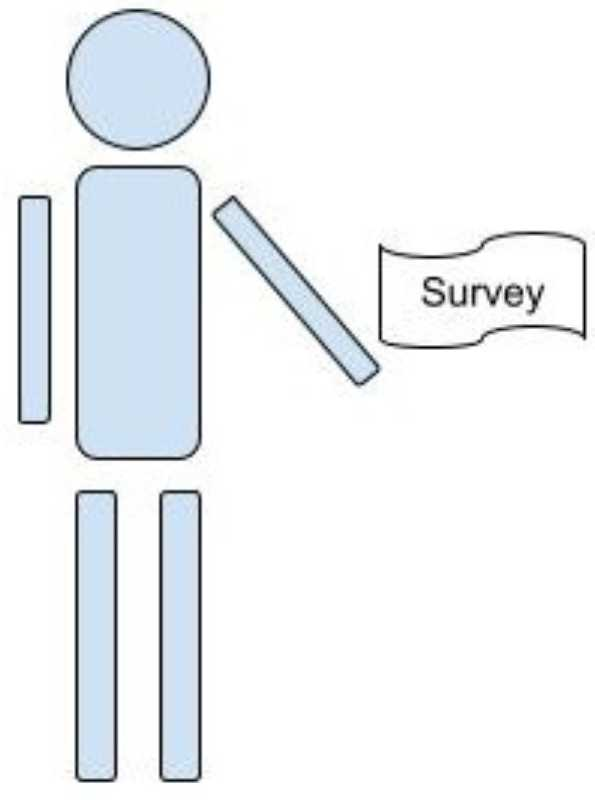
\includegraphics[width=0.5\textwidth]{static_figures/survey_man.jpg}
    }
    \only<2->{
    
\includegraphics[width=0.5\textwidth]{static_figures/survey_crazy_man.jpg}
    }
}{
    \centering
    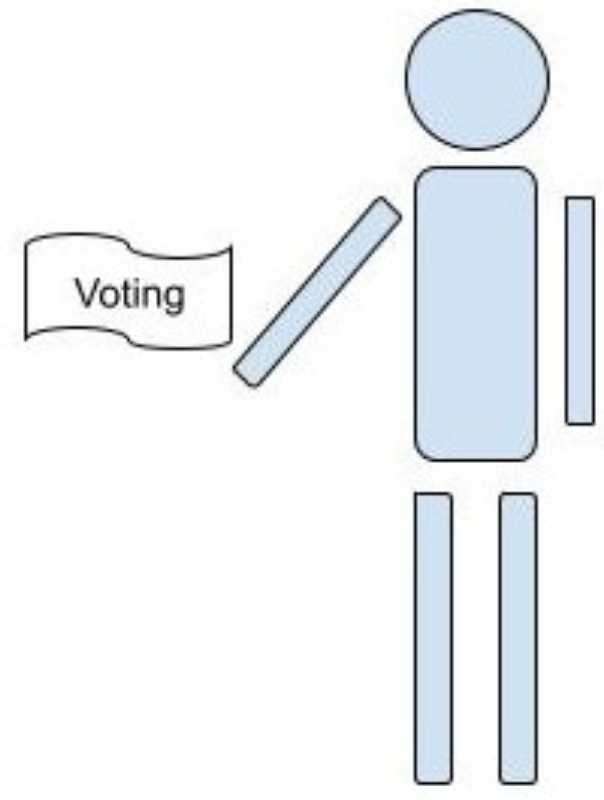
\includegraphics[width=0.5\textwidth]{static_figures/voting_man.jpg}
}

\splitpage{
    \centering
    Observe $(\x_s, y_s)$ for $s = 1, \ldots, \nsur$\\
}{
    \centering
    Observe $\x_p$ for $p = 1, \ldots, \ntar$\\
}

\onslide<2->{
\textbf{The problem is that the populations are very different.}
}

\onslide<3->{
    Our survey results may be biased.

    How can we use the covariates
    to say something about the target responses?
}
%
\end{frame}

%%%%%%%%%%%%%%%%%%%%%%%%%%%%%%%%%%%%%%%%%%%%%%%%%%%%%%%
%%%%%%%%%%%%%%%%%%%%%%%%%%%%%%%%%%%%%%%%%%%%%%%%%%%%%%%
%%%%%%%%%%%%%%%%%%%%%%%%%%%%%%%%%%%%%%%%%%%%%%%%%%%%%%%

\begin{frame}[t]{Two approaches}

We want $\mu := \meantar \y_p$, but don't observe $\y_p$ in the target population.

\begin{itemize}
    \item Assume $p(y | x)$ is the same in both populations,
    \item But the distribution of $x$ may be different in the survey and target.
\end{itemize}
%

\splitpage{
    \centering
    \textbf{Calibration weighting}
}{
    \centering
    \textbf{Bayesian hierarchical modeling (MrP)}
}

\splitpage{
    \centering
    Choose ``calibration weights'' $w_s$\\
    (e.g.~raking weights)
}{
    \centering
    Choose a model $\p(\y | x, \theta)$ and prior $\p(\theta)$\\
    (e.g.~Hierarchical logitstic regression)
}

\splitpage{
    \centering
    $\muhat_{\cal} = \meansur w_s y_s$
}{
    \centering
    Take $\yhat_p = \expect{\p(\theta \vert \textrm{Survey data})}{\y | \x_p}$ and\\
    $\muhat_{\mrp} = \meantar \yhat_p$
}

\splitpage{
    \centering
    Dependence on $\y_s$ is obvious\\
    ($\w_s$ typically chosen using only $\x$)
}{
    \centering
    Dependence on $\y_s$ very complicated\\
    (Typically via MCMC draws from $\p(\theta \vert \textrm{Survey data})$)
}

\splitpage{
    \centering
    Weights give interpretable diagnostics:
    %
    \begin{itemize}
        \item Frequentist variability
        \item Partial pooling
        \item Regressor balance
    \end{itemize}
    %
}{
    \centering
    \textbf{Black box}
}

We open the MrP black box, and provide versions of all these diagnostics,
for nonlinear hierarchical models fit with MCMC.

\end{frame}